\documentclass[aspectratio=169,11pt]{beamer}
\usetheme{default}
\usepackage{tikz,graphicx,amsmath,booktabs}
\usetikzlibrary{positioning,arrows.meta}
\definecolor{ink}{HTML}{17324D}\definecolor{accent}{HTML}{26749D}\definecolor{pale}{HTML}{EAF3F7}
\setbeamercolor{normal text}{fg=ink,bg=white}\setbeamercolor{frametitle}{fg=ink}\setbeamercolor{structure}{fg=accent}
\setbeamertemplate{navigation symbols}{}\setbeamertemplate{footline}[frame number]
\tikzset{box/.style={draw=accent,fill=pale,rounded corners,align=center,minimum height=11mm,minimum width=25mm},arr/.style={-{Stealth},thick,accent}}
\newcommand{\smallnote}[1]{{\scriptsize\color{gray}#1}}
\begin{document}
\begin{frame}{Which Exposure Matters?\hfill\small Introduction}
\large Can an image model combine familiar ideas it rarely sees together?
\begin{columns}[c]\column{.56\textwidth}\normalsize A diffusion model starts with noise and learns to produce an image matching a condition. We study how the \textbf{composition of training examples} affects this ability.\vspace{2mm}\\
\scriptsize Kanishak Mittal \texttt{cs24b1017@iiitr.ac.in}\\ Aryan Tripathi \texttt{ad24b1010@iiitr.ac.in}\\ Nikhil Tomar \texttt{cs24b1041@iiitr.ac.in}\\ Vansh Rathore \texttt{cs24b1061@iiitr.ac.in}
\column{.42\textwidth}\centering
\includegraphics[width=.29\textwidth]{assets/noise-3.png} $\rightarrow$ 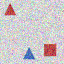
\includegraphics[width=.29\textwidth]{assets/noise-1.png} $\rightarrow$ 
\includegraphics[width=.29\textwidth]{assets/noise-0.png}\\\smallnote{Illustrative forward-noising images shown in reverse order; not model outputs.}\end{columns}\end{frame}
\begin{frame}{Literature survey: what is missing?}\begin{itemize}
\item \textbf{DDPM} learns generation by reversing noise corruption (Ho et al., 2020).
\item \textbf{Latent diffusion} scales conditional generation in compressed representations (Rombach et al., 2022).
\item \textbf{Compositional diffusion} combines learned concept models (Liu et al., 2022).
\item \textbf{MOSAIC} investigates compositional image generation (Jeong et al., 2026).
\end{itemize}\begin{block}{Our question}How much does \emph{joint training exposure} matter when individual concept frequencies are held similar?\end{block}
\smallnote{arXiv:2006.11239; arXiv:2112.10752; arXiv:2206.01714; proceedings.mlr.press/v306/jeong26b.html.}\end{frame}
\begin{frame}{Research hypothesis: parts versus combinations}\centering
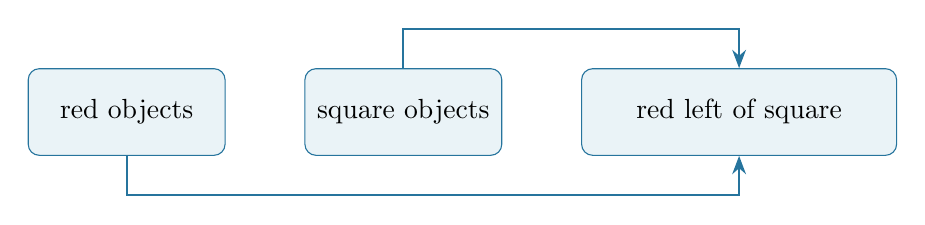
\begin{tikzpicture}[node distance=10mm]\node[box] (a) {red objects}; \node[box,right=of a] (b) {square objects}; \node[box,right=of b,minimum width=40mm] (c) {red left of square};\draw[arr] (a.south) -- ++(0,-.5) -| (c.south); \draw[arr] (b.north) -- ++(0,.5) -| (c.north);\end{tikzpicture}
\vspace{3mm}\begin{itemize}\item \textbf{H1:} joint exposure affects success even when individual concept frequencies stay similar.\item \textbf{H2:} harder scenes may affect success more than color imbalance in the controlled toy setting.\end{itemize}\smallnote{Research hypotheses, not conclusions. Distinct objects are required for binary relations.}\end{frame}
\begin{frame}{Methodology: an experiment, not just a benchmark}\centering
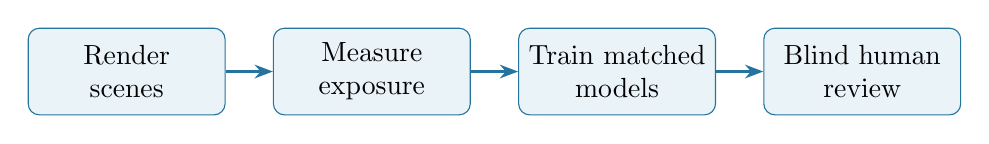
\begin{tikzpicture}[node distance=6mm]\node[box] (a) {Render\\ scenes};\node[box,right=of a] (b) {Measure\\ exposure};\node[box,right=of b] (c) {Train matched\\ models};\node[box,right=of c] (d) {Blind human\\ review};\draw[arr] (a)--(b);\draw[arr] (b)--(c);\draw[arr] (c)--(d);\end{tikzpicture}
\vspace{4mm}\begin{columns}[T]\column{.52\textwidth}\textbf{Control}: synthetic objects, attributes and relations let us count what examples contain.\column{.46\textwidth}\textbf{Compare}: separate exposure to ingredients from exposure to the full combination.\end{columns}\vspace{3mm}\smallnote{Main rule-exposure study remains in design validation; networking prototype streams scenes over TCP; Localhost: 300k scenes per batch, 1,060--1,082 scenes/s. SSH tunnel: 300 scenes, 582--926 scenes/s; GPU idle unmeasured.}\end{frame}
\begin{frame}{Model architecture: learning to reverse noise}\centering
\resizebox{.95\textwidth}{!}{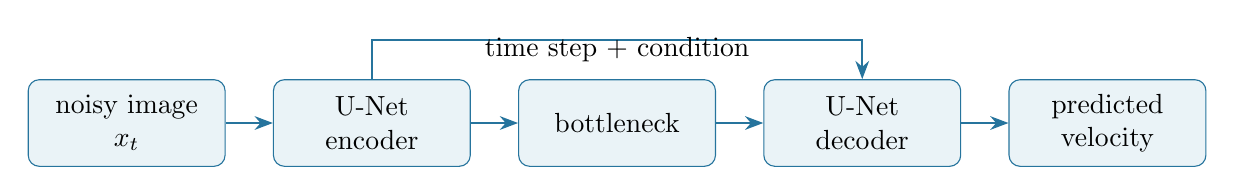
\begin{tikzpicture}[node distance=6mm]\node[box] (x) {noisy image\\$x_t$};\node[box,right=of x] (e) {U-Net\\encoder};\node[box,right=of e] (b) {bottleneck};\node[box,right=of b] (d) {U-Net\\decoder};\node[box,right=of d] (v) {predicted\\velocity};\draw[arr](x)--(e);\draw[arr](e)--(b);\draw[arr](b)--(d);\draw[arr](d)--(v);\draw[arr](e.north) -- ++(0,.5) -| (d.north);\node[above=.1cm of b] {time step + condition};\end{tikzpicture}}
\vspace{4mm}\[x_t=\sqrt{\bar\alpha_t}x_0+\sqrt{1-\bar\alpha_t}\,\epsilon\]\small Forward process adds noise; the network predicts the denoising target. Repeated reverse steps generate an image.\end{frame}
\begin{frame}{Dataset: a controlled synthetic world}\begin{columns}[c]\column{.52\textwidth}\begin{itemize}\item Simple colored shapes with known object attributes.\item Relations: \emph{left of} and \emph{above}; ground truth from scene metadata.\item Pilot: four cells, 200 fixed scenes per cell.\item Rule study: 57 candidate conditions, still under validation.\end{itemize}\column{.45\textwidth}\centering
\includegraphics[width=.75\textwidth]{assets/synthetic-example.png}\\\smallnote{Illustrative rendered scene; not a generated prediction.}\end{columns}\end{frame}
\begin{frame}{Experimental setup: controlled 2 $\times$ 2 pilot}\centering\begin{tabular}{lcc}\toprule & Balanced & Imbalanced\\\midrule Low complexity & 2 objects; 50:50 & 2 objects; 90:10\\ High complexity & 3 objects; 50:50 & 3 objects; 90:10\\\bottomrule\end{tabular}
\vspace{4mm}\begin{itemize}\item Four fresh PilotUNet models; 500,000 updates each; same training budget.\item Generate 16 images per cell: red/blue target $\times$ eight paired noise seeds.\item Primary outcome: is the requested-color circle present?\end{itemize}\smallnote{One matched training-seed block; separate second block underway. Object count is secondary, not an input condition.}\end{frame}
\begin{frame}{Quantitative results: target circle in 64 images}\centering\begin{tabular}{lrrr}\toprule Condition & Yes & No & Unresolved\\\midrule Low / balanced &16&0&0\\ Low / imbalanced &15&0&1\\ High / balanced &14&2&0\\ High / imbalanced &14&1&1\\\bottomrule\end{tabular}\vspace{3mm}\begin{block}{Descriptive contrast in this image set}Complexity drop: 6.25--12.5 percentage points; imbalance drop: $-3.125$ to $3.125$ points.\end{block}\smallnote{Ranges assign uncertain responses both ways; not confidence intervals. Four CSVs were identical, so independent authorship is unverified.}\end{frame}
\begin{frame}{Qualitative results: looking beyond a score}\begin{columns}\column{.5\textwidth}\centering
\includegraphics[width=.47\textwidth]{assets/review-0003.png}\\\textbf{Sample 0003}\\\small Target-circle answer: yes; exactly two objects: yes.\column{.5\textwidth}\centering
\includegraphics[width=.47\textwidth]{assets/review-0001.png}\\\textbf{Sample 0001}\\\small Target-circle answer: unsure; object-count answers: no.\end{columns}\vspace{3mm}\smallnote{Generated pilot images selected to show differing review outcomes; not representative performance estimates. No paired ground truth exists for stochastic generation.}\end{frame}
\begin{frame}{Ablation and failure cases}\begin{itemize}\item The $2\times2$ pilot changes scene complexity and color balance under matched settings; a \textbf{data-factor comparison}, not a U-Net component ablation.\item Experimental checker answered 46 of 64 target-circle questions; it abstained on all three reviewed ``no'' cases and both uncertain cases.\item This sample cannot estimate its false-accept rate. A foreground segmenter reached IoU 0.935 on 100 blurred synthetic scenes; its rule adapter answered 54/300 reviewed images versus 95/300 for baseline.\end{itemize}\begin{alertblock}{Remaining design issue}Legacy relation exposure $\approx0.99927$; min-KL at uniform is a no-op. A replacement design and checker still need validation.\end{alertblock}\end{frame}
\begin{frame}{Discussion: what do these findings mean?}\begin{columns}[T]\column{.5\textwidth}\textbf{Observed}\begin{itemize}\item Pilot shows how complexity and imbalance can be compared.\item Observed complexity contrast exceeds imbalance contrast for these 64 images.\end{itemize}\column{.48\textwidth}\textbf{Not established}\begin{itemize}\item Generalization across training seeds or datasets.\item Checker validity on failures.\item Whether full-rule exposure independently causes success.\end{itemize}\end{columns}\smallnote{$\Gamma_{\log}=\log\mathrm{RSR}-\sum_p\log c_p$; the earlier logit identity criticism was retracted. Identical CSVs do not prove independent authorship.}\end{frame}
\begin{frame}{Conclusion and future work}\begin{itemize}\item \textbf{Contribution}: a framework to separate exposure to constituents from exposure to their combinations.\item \textbf{Current status}: exploratory pilot and audit complete; Stage 0 has not passed.\item \textbf{Next}: finish the second model-seed block and review, validate the checker, and resolve design identifiability before testing H1.\end{itemize}\begin{block}{Takeaway}Knowing individual pieces need not guarantee the requested composition; we investigate how training exposure changes that.\end{block}\smallnote{Repository: github.com/Space-Dev0/muadib}\end{frame}
\end{document}
